\documentclass[
    11pt,
    oneside, %  comment to switch to alternatig margins (for printed layout)
    english,
    singlespacing, % Single line spacing, alternatives: onehalfspacing or doublespacing
%draft, % Uncomment to enable draft mode (no pictures, no links, overfull hboxes indicated)
%nolistspacing, % If the document is onehalfspacing or doublespacing, uncomment this to set spacing in lists to single
%liststotoc, % Uncomment to add the list of figures/tables/etc to the table of contents
%toctotoc, % Uncomment to add the main table of contents to the table of contents
parskip, % Uncomment to add space between paragraphs
%nohyperref, % Uncomment to not load the hyperref package
    headsepline, % Uncomment to get a line under the header
%chapterinoneline, % Uncomment to place the chapter title next to the number on one line
%consistentlayout, % Uncomment to change the layout of the declaration, abstract and acknowledgements pages to match the default layout
]{MastersDoctoralThesis}

\usepackage[utf8]{inputenc}
\usepackage[T1]{fontenc}
\usepackage[nodayofweek]{datetime}
\usepackage{mathpazo}
%\usepackage{fontspec}
%\setmonofont{Consolas}

%\usepackage{pgfgantt}
\usepackage[backend=bibtex,style=vancouver,natbib=true]{biblatex} % Use the bibtex backend with the authoryear citation style (which resembles APA)

\addbibresource{biblio.bib}

\usepackage[autostyle=true]{csquotes}
\usepackage{tikz}
\usetikzlibrary{shapes.misc, arrows.meta}
\usepackage{amsmath}
\usepackage{amsthm}
\usepackage{textcomp}
\usepackage{color}
\usepackage{markdown}
\usepackage{wasysym}
\usepackage{amssymb}
\usetikzlibrary{arrows,positioning}
%\tikzset{
%%Define standard arrow tip
%    >=stealth',
%%Define style for boxes
%    punkt/.style={
%        rectangle,
%        rounded corners,
%        draw=black, thick,
%        text width=6.5em,
%        minimum height=2em,
%        text centered},
%% Define arrow style
%    pil/.style={
%        ->,
%        thick,
%        shorten <=2pt,
%        shorten >=2pt,}
%}
\geometry{
    paper=a4paper,
    inner=2.5cm,
    outer=3.8cm,
    bindingoffset=.5cm,
    top=1.5cm,
    bottom=1.5cm,
%showframe, % Uncomment to show how the type block is set on the page
}

% personal macros

\newcommand{\citeTODO}{[\scriptsize{\textit{\textsc{CITATION NEEDED}}}\normalsize]}
\newdateformat{daymonth}{
    \ordinal{DAY}\ of \monthname[\THEMONTH]
}
\newcommand{\monthdate}[2]{ \daymonth\formatdate{#1}{#2}{2022}}
% TODO find a nice definition format
\theoremstyle{definition}
\newtheorem{definition}{Definition}
\providecommand*\definitionautorefname{Definition}
\providecommand*{\listingautorefname}{Listing}


%
%\newcommand{\thickerhline}{
%    \setlength{\arrayrulewidth}{.11.6.105em}
%    \hline
%    \setlength{\arrayrulewidth}{.05em}
%}

%\thesistitle{Exploring Trustless Licensing} % print with \ttitle
\thesistitle {Confis: A Framework for Authoring and Querying Machine-Readable Legal Agreements}
\supervisor{Prof. William J. \textsc{Knottenbelt}} % print with \supname
\marker{Dr. Paul A. \textsc{Bilokon}}
\degree{MEng Computing} % print with \degreename
\author{Nicolás \textsc{D'Cotta}} % print with \authorname
\addresses{} % print with \addressname

\subject{Computer Science} % Your subject area, this is not currently used anywhere in the template, print it elsewhere with \subjectname
\keywords{} % TODO fill - print with \keywordnames
\university{\href{https://www.imperial.ac.uk/}{Imperial College London}} % Your university's name and URL, this is used in the title page and abstract, print it elsewhere with \univname
\department{\href{https://www.imperial.ac.uk/computing}{Department of Computing}} % Your department's name and URL, this is used in the title page and abstract, print it elsewhere with \deptname
\group{\href{https://researchgroup.university.com}{Research Group Name}} % Your research group's name and URL, this is used in the title page, print it elsewhere with \groupname
\faculty{\href{https://faculty.university.com}{Faculty of Engineering}} % Your faculty's name and URL, this is used in the title page and abstract, print it elsewhere with \facname

\AtBeginDocument{
    \hypersetup{pdftitle=\ttitle} % Set the PDF's title to your title
    \hypersetup{pdfauthor=\authorname} % Set the PDF's author to your name
    \hypersetup{pdfkeywords=\keywordnames} % Set the PDF's keywords to your keywords
}


\begin{document}
    \usemintedstyle{tango}
    \frontmatter
    \pagestyle{plain}

%----------------------------------------------------------------------------------------
%	TITLE PAGE
%----------------------------------------------------------------------------------------

    \begin{titlepage}
        \begin{center}

            \vspace*{.06\textheight}
            {\scshape\LARGE \univname\par}\vspace{1.5cm}
            % TODO restore for report
            \textsc{\Large MEng Final Year Project}\\[0.5cm]

            \HRule \\[0.4cm]
            {\huge \bfseries \ttitle\par}\vspace{0.4cm} % Thesis title
            \HRule \\[1.5cm]

            \begin{minipage}[t]{0.4\textwidth}
                \begin{flushleft}
                    \large
                    \emph{Author:}\\
                    \href{https://nico.dcotta.eu}{\authorname}
                \end{flushleft}
            \end{minipage}
            \begin{minipage}[t]{0.4\textwidth}
                \begin{flushright}
                    \large
                    \emph{Supervisor:} \\
                    \href{https://www.doc.ic.ac.uk/~wjk/}{\supname} \\[0.4 cm]
                    \emph{Second Marker:} \\
                    \href{https://www.imperial.ac.uk/people/paul.bilokon01}{\markername}
                \end{flushright}
            \end{minipage}\\[3cm]

            \vfill
            \large \textit{A report submitted in fulfillment of the requirements\\ for the degree of \degreename}\\[0.3cm] % University requirement text
            \textit{in the}\\[0.4 cm]
            \facname \\ \deptname\\[2 cm]

            \vfill

            {\large \today}\\[4cm] % Date
%\includegraphics{Logo} % University/department logo - uncomment to place it

            \vfill
        \end{center}
    \end{titlepage}


    \begin{abstract}
        \addchaptertocentry{\abstractname} % Add the abstract to the table of contents

        % make it clear why you I am trying to operationalise contracts
        % - make it easier to exploit digital form of the contract
        % - give people an understanding of capabilities, exposures, obligations wrt contracts

        % no technologies succeed at helping us understand a contract
        % lots of automation tech around contracts but it focuses on bureaucratic overheads (such as signing, version control, and proof of existence).


        For more than four thousand years, humankind has utilised contracts to govern economic activity.
        Since their conception in ancient times, they have been represented as clauses of natural language and how we reason about them has remained unchanged, despite technological leaps and civilization's dependence on them.
        In the last few decades, since the seminal work on smart contracts by Szabo in 1997, the benefits of formalising and automating contracts have become increasingly obvious.
        Such benefits include making it easier for parties to understand the legal constraints they are under, as well as the capabilities they have.

        % missing direction of travel at the end of 1st paragrapgh

        % there are lots of contracts -> they are nat language -> how we reason about them has remained unchanged since their conception 3 thousand years ago


        Rather than replacing existing legal infrastructure, some new technologies like blockchain-based smart contracts have created a new class of self-enforcing software systems which mostly revolve around financial products.
        Other, more logic-based attempts to automate reasoning with legal documents are very specialist and require understanding of advanced topics, such as logic programming, linear temporal logic, or the event calculus;
        and are not self-contained solutions.
        This lack of accessibility of existing technologies means that they have not seen practical adoption in industry.

        This project introduces \textbf{\emph{Confis}}, a Kotlin-based accessible language that specifies legal agreements and immediately answers complex queries.
%        Its features include converting documents back to plain English, an intelligent editor with a live preview, and a user interface for performing complex queries on documents as they are written.
        Contracts are written as stand-alone scripts inside a fully-capable editor based on IntelliJ IDEA, inside which a live preview displays a plain English render of the encoded agreement.
        In stark contrast with the state of the art, Confis does not require engineering, logical, nor legal expertise for its effective use.
        A graphical UI allows making questions involving parties' legal capabilities and their compliance, such as \emph{`What needs to happen for my landlord evict me?'} or \emph{`Has the seller breached our agreement?'} -- which Confis is able to answer in plain English.


        % something in this technical paragraph about architecture ^
        % showcase your technical achievement!

%        The result is an end-to-end framework that provides abstractions that successfully represents a broad range of contracts, comparable to Symboleo or The Accord Project, except with a strong focus on accessibility and ease-of-use aimed at industry.
%        Simple and easier to learn abstractions are brought forward by compromising mainly on language expressiveness -- and therefore in the complexity of the contracts that can be represented.

        % Last paragraph is kind of queries
        Overall, this project operationalises legal agreements by providing the industry with relevant and pragmatic tools.
        By formalising the fewest key abstractions, we prove it successfully represents common classes of contracts (such as licenses and sales agreements) much like Symboleo or The Accord project -- except with a strong focus on accessibility and through a self-contained solution.
        Confis also succeeds at avoiding exposing advanced complexities that hinder its accessibility, by compromising on language expressiveness.
        We show this accessibility is at the price of not being able to formalise some more specific legal scenarios, which limits the range of contracts Confis can specify.

        Next steps include communicating with other services for them to be aware of their legal capabilities (rather than relying on legal advice across teams inside an organisation), as well as improving the compromise between the contracts that can be represented and the complexity of the language.
        % specify how you built on top of another lang as an internal DSL

        % last para did you manage succesfully?? what about the future of contracts in general
        % what works what does not work
        % general outlook

        % what case studies

    \end{abstract}


    \begin{acknowledgements}
        \addchaptertocentry{\acknowledgementname} % TODO write akcnowledgements
        I would like to thank William, my supervisor\dots.
    \end{acknowledgements}

    \tableofcontents
    \listoffigures
    \listoftables
    \listoflistings

%    \setlength{\parskip}{\medskipamount}
    \setlength{\parindent}{0pt}


    \mainmatter % Begin numeric (1,2,3...) page numbering

    \pagestyle{thesis} % Return the page headers back to the "thesis" style


    \chapter{Introduction}\label{ch:introduction}

\section{The Hassle of Enterprise Legal Agreements}\label{sec:intro:legal-hassle}

Businesses are routinely bound by legal agreements to each other and those agreements give them constraints with respect to
the legal boundaries they can operate within.
While compliance with the agreement is typically in the interest of all parties involved, it is difficult
to achieve: legal advice - most commonly costly and billed by the hour - must be sought out to
deal with any non-routine situation.

Additionally, even when an agreement is being complied with by all, parties must be able to prove they are compliant,
leading to large amounts of unstructured documents of audit trails.\\

I suggest automating some hassles of legal agreement compliance, audit and verification, by encoding a contract
in a machine-readable format and enable querying it and logging interactions.
The goals are:
\begin{itemize}
    \item Minimising costs in legal advice by allowing a business to 'ask questions' about the legal boundaries within
    which they are able to operate.
    \item Enabling secure audit trails that all parties involved in the agreement can trust in order to prove
    compliance (or lack thereof!).
\end{itemize}

\\ \\
Thanks for assisting to my TED talk~\citeTODO.

    \chapter{Background}\label{ch:background}


\section{Cryptography Primitives}\label{sec:cryptography}

\subsection{Hash Functions}\label{subsec:crypto:hash}

Hash functions are cryptographic functions designed to behave like random
functions~\cite{smart2016randomOracleModel}.
When building a security proof, they can be assumed to have the following properties~\cite{smart2016randomOracleModel,
    smart2016hashFunctions}:
% FIXME needs references
\begin{description}
    \item[Determinism] A hash function always produces the same output for the same input
    \item[One-way] It is computationally impossible to compute the preimage for some output of a hash function
    \item[Uniformity] Outputs of a hash function are expected to be uniformly distributed.
    In practice, the output space of a hash function is finite, so \textit{collisions} (where two inputs produce the
    same output) are possible, but uniformity ensures this is an unlikely scenario.
\end{description}

\subsection{Symmetric key cryptography}

% TODO will i need this

\subsection{Public Key Cryptography}\label{subsec:crypto:pubkey}

In public key cryptography, two communicating parties (say Alice and Bob) can communicate privately by using pairs of
numbers that are related mathematically and which allow converting cleartext into cyphertext and
back~\cite{smart2016publicKey}.
This pair of numbers is called an asymmetric keypair, and is composed of a \textbf{public key} $e$ and a \textbf{private
key} $d$.\\

In this example, if Alice wishes to communicate with Bob, Bob can generate a keypair $(d, e)$ and publish $e$.
Alice can then encrypt her cleartext with $e$, and only Bob will be able to decrypt it (because only Bob knows $d$).

\begin{figure}[th]
    \centering
    \tikzset{every picture/.style={line width=0.75pt}} %set default line width to 0.75pt
    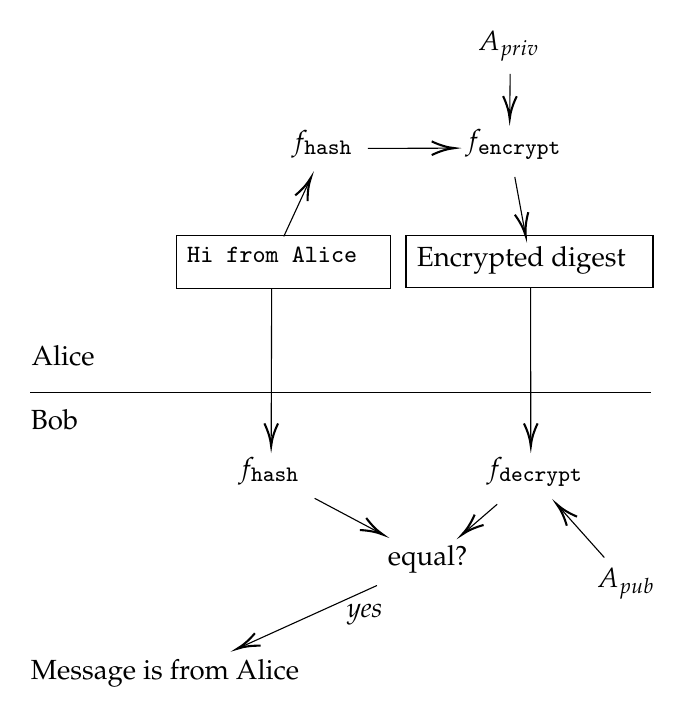
\begin{tikzpicture}[x=0.75pt,y=0.75pt,yscale=-1,xscale=1]
%uncomment if require: \path (0,355); %set diagram left start at 0, and has height of 355

%Straight Lines [id:da017592532205451983]
        \draw    (60.54,179.69) -- (359.87,179.69) ;

% Text Node
        \draw    (131,104) -- (234,104) -- (234,129.67) -- (131,129.67) -- cycle ;
        \draw (135,108.67) node [anchor=north west][inner sep=0.75pt]   [align=left] {\small \texttt{Hi from Alice}};
% Text Node
        \draw (185.33,52.33) node [anchor=north west][inner sep=0.75pt]   [align=left] {$\displaystyle f_{\texttt{hash}}$};
% Text Node
        \draw (275,4.33) node [anchor=north west][inner sep=0.75pt]   [align=left] {$\displaystyle A_{priv}$};
% Text Node
        \draw (332.33,263.33) node [anchor=north west][inner sep=0.75pt]   [align=left] {$\displaystyle A_{pub}$};
% Text Node
        \draw (269,52) node [anchor=north west][inner sep=0.75pt]   [align=left] {$\displaystyle f_{\texttt{encrypt}}$};
% Text Node
        \draw    (241.67,104) -- (360.67,104) -- (360.67,129.33) -- (241.67,129.33) -- cycle ;
        \draw (245.67,108.33) node [anchor=north west][inner sep=0.75pt]   [align=left] {Encrypted digest};
% Text Node
        \draw (60,156) node [anchor=north west][inner sep=0.75pt]   [align=left] {Alice};
% Text Node
        \draw (59.67,186.67) node [anchor=north west][inner sep=0.75pt]   [align=left] {Bob};
% Text Node
        \draw (159.67,209.67) node [anchor=north west][inner sep=0.75pt]   [align=left] {$\displaystyle f_{\texttt{hash}}$};
% Text Node
        \draw (279.33,209.67) node [anchor=north west][inner sep=0.75pt]   [align=left] {$\displaystyle f_{\texttt{decrypt}}$};
% Text Node
        \draw (231.67,252.33) node [anchor=north west][inner sep=0.75pt]   [align=left] {equal?};
% Text Node
        \draw (59.67,307.33) node [anchor=north west][inner sep=0.75pt]   [align=left] {Message is from Alice};
% Text Node
        \draw (208.67,280.33) node [anchor=north west][inner sep=0.75pt]   [align=left] {\textit{{ yes}}};
% Connection
        \draw    (182.78,104.67) -- (195.03,78.15) ;
        \draw [shift={(195.87,76.33)}, rotate = 114.8] [color={rgb, 255:red, 0; green, 0; blue, 0 }  ][line width=0.75]    (10.93,-3.29) .. controls (6.95,-1.4) and (3.31,-0.3) .. (0,0) .. controls (3.31,0.3) and (6.95,1.4) .. (10.93,3.29)   ;
% Connection
        \draw    (223.33,62.25) -- (263,62.11) ;
        \draw [shift={(265,62.1)}, rotate = 179.79] [color={rgb, 255:red, 0; green, 0; blue, 0 }  ][line width=0.75]    (10.93,-3.29) .. controls (6.95,-1.4) and (3.31,-0.3) .. (0,0) .. controls (3.31,0.3) and (6.95,1.4) .. (10.93,3.29)   ;
% Connection
        \draw    (294.1,76) -- (298.98,102.37) ;
        \draw [shift={(299.35,104.33)}, rotate = 259.5] [color={rgb, 255:red, 0; green, 0; blue, 0 }  ][line width=0.75]    (10.93,-3.29) .. controls (6.95,-1.4) and (3.31,-0.3) .. (0,0) .. controls (3.31,0.3) and (6.95,1.4) .. (10.93,3.29)   ;
% Connection
        \draw    (291.87,26.33) -- (291.66,46) ;
        \draw [shift={(291.64,48)}, rotate = 270.59] [color={rgb, 255:red, 0; green, 0; blue, 0 }  ][line width=0.75]    (10.93,-3.29) .. controls (6.95,-1.4) and (3.31,-0.3) .. (0,0) .. controls (3.31,0.3) and (6.95,1.4) .. (10.93,3.29)   ;
% Connection
        \draw    (176.96,129.67) -- (176.72,203.67) ;
        \draw [shift={(176.71,205.67)}, rotate = 270.19] [color={rgb, 255:red, 0; green, 0; blue, 0 }  ][line width=0.75]    (10.93,-3.29) .. controls (6.95,-1.4) and (3.31,-0.3) .. (0,0) .. controls (3.31,0.3) and (6.95,1.4) .. (10.93,3.29)   ;
% Connection
        \draw    (301.69,129.33) -- (301.81,203.67) ;
        \draw [shift={(301.81,205.67)}, rotate = 269.91] [color={rgb, 255:red, 0; green, 0; blue, 0 }  ][line width=0.75]    (10.93,-3.29) .. controls (6.95,-1.4) and (3.31,-0.3) .. (0,0) .. controls (3.31,0.3) and (6.95,1.4) .. (10.93,3.29)   ;
% Connection
        \draw    (197.67,230.82) -- (228.87,247.4) ;
        \draw [shift={(230.63,248.33)}, rotate = 207.98] [color={rgb, 255:red, 0; green, 0; blue, 0 }  ][line width=0.75]    (10.93,-3.29) .. controls (6.95,-1.4) and (3.31,-0.3) .. (0,0) .. controls (3.31,0.3) and (6.95,1.4) .. (10.93,3.29)   ;
% Connection
        \draw    (285.62,233.67) -- (270.15,247.03) ;
        \draw [shift={(268.64,248.33)}, rotate = 319.18] [color={rgb, 255:red, 0; green, 0; blue, 0 }  ][line width=0.75]    (10.93,-3.29) .. controls (6.95,-1.4) and (3.31,-0.3) .. (0,0) .. controls (3.31,0.3) and (6.95,1.4) .. (10.93,3.29)   ;
% Connection
        \draw    (227.67,272.83) -- (162.1,302.51) ;
        \draw [shift={(160.28,303.33)}, rotate = 335.64] [color={rgb, 255:red, 0; green, 0; blue, 0 }  ][line width=0.75]    (10.93,-3.29) .. controls (6.95,-1.4) and (3.31,-0.3) .. (0,0) .. controls (3.31,0.3) and (6.95,1.4) .. (10.93,3.29)   ;
% Connection
        \draw    (337.23,259.33) -- (315.66,235.16) ;
        \draw [shift={(314.33,233.67)}, rotate = 48.25] [color={rgb, 255:red, 0; green, 0; blue, 0 }  ][line width=0.75]    (10.93,-3.29) .. controls (6.95,-1.4) and (3.31,-0.3) .. (0,0) .. controls (3.31,0.3) and (6.95,1.4) .. (10.93,3.29)   ;

    \end{tikzpicture}
    \decoRule
    \caption[Asymmetric signing scheme]{An asymmetric key signing scheme where Bob is able to verify only Alice could have written '\texttt{Hi from Alice}'}
    \label{fig:pubkey-signing}
\end{figure}

Conversely, the same keypair can be used by Bob to send a message to Alice where Alice can verify that only Bob
could have written the message.
This is called \textit{signing}~\cite{smart2016signatures} and, more generally, it allows a sender of a message to
prove they are the authors of the message to a recipient.
An example of a signing scheme can be seen in Figure~\ref{fig:pubkey-signing}.

\subsection{Secure Digital Timestamps}\label{subsec:crypto:timestamps}
% TODO citation for definiton
\textit{Trusted (digital) timestamping} is the process of securely proving that a document (for our purposes, a blob of bytes) was
created, was modified at, or existed at a certain point in time.
% TODO citation for widely used
In industry this is commonly implemented by trusting a Time Stamping Authority (TSA)~\cite{timestamps_tsp_rfc} that
signs (see~\nameref{subsec:crypto:pubkey}) a concatenation of the hash of the document and a timestamp representing some
time $t$.
Therefore a party that trusts the TSA to provide the right timestamp can verify that, when the TSA made the signature,
the current time was $t$.
\\

This method can be used for confidential data because the TSA does not perform the hashing of the original document
themselves - they are exposed only to its digest.

Additionally, the requester of the timestamp cannot deny they were not in possession of the original data at the time
% TODO verify statement
$t$ given by the timestamp, because it was them that produced its hash digest.

\subsubsection{Decentralised Timestamps}

Secure timestamps can also be achieved without relying on trusted parties by publishing
the document digest to a blockchain~\cite{gipp2015timestamps_btc}: blocks are public and cannot be tampered with (see~\nameref{subsec:btc:pow}), so
putting a signed digest in a block shows that the signer knew the original document at the time the block was accepted
by the network.


\section{Bitcoin Protocol}\label{sec:bitcoin}

Blockchain technology was introduced by~\cite{nakamoto2008bitcoin} as a decentralised system allowing for electronic
cash payments.
Blockchains are immutable distributed ledgers where participants' balances can be verified by every other participant,
and it is computationally hard to tamper with balances to perform attacks (such as performing a transaction where a
participant spends more funds than what they own). \\
I will provide a brief overview of how Bitcoin provides these guarantees.

\subsection{Transactions}\label{subsec:btc:txs}

\cite{nakamoto2008bitcoin} defines an \textit{electronic coin} as a chain of signatures: a payer can use their private
key, the hash of the previous transaction, and the payee's public key to create a signed hash that can be verified by
the payee (and used by them for \textit{their} next transaction).
This is illustrated in Figure~\ref{fig:bitcoin-tx}.

\begin{figure}[th]
    \centering
    \includegraphics[width=0.8\columnwidth]{figures/bitcoin-tx}
    \caption[Bitcoin coin ownership transfer]{Transfer of ownership signature chain, from~\cite{nakamoto2008bitcoin}}
    \label{fig:bitcoin-tx}
\end{figure}

This ensures that, as long as a participants sign transactions at most once:
\begin{itemize}
    \item By verifying the chain of signatures, every participant can verify which participant owns which coin
    \item Only the owner of a coin can initiate a transaction with that coin
\end{itemize}

Bitcoin enforces that participants can only sign transactions once thanks to its proof-of-work
(see~\ref{subsec:btc:pow}) algorithm.

\subsection{Proof-Of-Work}\label{subsec:btc:pow}

Bitcoin ensures 'unique signatures' in transactions by grouping transactions in immutable, public \textit{blocks}.
Participants can then verify a payer has not signed a hash of a single transaction twice by looking at all existing
transactions.\\

Blocks are made immutable by including in them a value (called a \textit{nonce}) and the hash of the previous block.
% TODO verify it is the hash of the entire block that must yield the zeroes (implementation detail really)
The protocol then accepts only blocks where the $n$ first bits of its hash are zeroes. \\

Thus, in order to publish a block a participant must do work to find a nonce such that the block's hash meets this
condition - then other participants can verify its validity with a single hash operation.
This guarantees that a block cannot be changed (ie, a new copy published) without redoing the computational work.
Because blocks are chained (they include the hash of the previous block), in order to modify a transaction in the past
an adversary needs to redo the computational work for every block since that transaction (see Figure
\ref{fig:bitcoin-blockchain}).
% TODO implementation of mining rewards
Additionally, participants that successfully find a suitable nonce and propose new blocks (also referred to as
\textit{miners}) are allowed to add a specific transaction to the block where they own a newly created coin (also
referred to as \textit{mining reward}).

\begin{figure}[th]
    \centering
    \includegraphics[width=0.8\columnwidth]{figures/bitcoin-blockchain}
    \caption[Two last blocks in a blockhain]{Two last blocks in a blockchain, from~\cite{nakamoto2008bitcoin}}
    \label{fig:bitcoin-blockchain}
\end{figure}


This model of consensus ensures that
\begin{itemize}
    \item Participants have a monetary incentive to stay honest with respect to the protocol
    \item An honest chain will out-compete an adversary's chain as long as the majority of computing power is honest
\end{itemize}

\subsection{Further details of the Bitcoin protocol}\label{subsec:btc.details}

While I provide a high-level overview of what makes the protocol function, there are many more details that combined
allow for more efficiency and usability:
\begin{itemize}
    \item Transactions may have several inputs and outputs, so participants can transfer amounts rather than single
    \textit{electronic coins}.
    Thus, a participant's balance is the sum of all the unspent outputs of previous transactions.
    \item By modifying how many of the leading bits of a blocks' hash must be zeroes, the average computation necessary
    to produce a new block can be adjusted by the protocol.
    \item By using Merkle Trees~\cite{merkle1980tree} transactions with fully spent transaction outputs can be discarded
    without breaking the block's hash.
    This allows compacting old blocks to reclaim disk space.
    \item A participant that does not wish to mine or hold a copy of the entire blockchain can still verify payments.
    It can keep a copy of the block headers of the longest chain and link a transaction to where it is on-chain and
    check that other network nodes have accepted it.
\end{itemize}
\\
For more information on all the workings of the Bitcoin protocol, please refer to~\cite{nakamoto2008bitcoin}.


\section{Ethereum Smart Contracts}\label{sec:ethereum}
% TODO idk to what extent I will need this?

Smart contracts were first formalised by~\cite{szabo1997smart-contracts} and implemented in~\cite{buterin2015ethereum}


\section{Licensing}
% TODO

\subsection{Dataset Licesing}
% TODO


\section{Zero-Knowledge Proofs}

An \textit{Interactive Proof} is a protocol where a verifier $V$ either \textit{accepts} or \textit{rejects} whether a
prover $P$ knows something~\cite{damgaard1998zk_protocols}.
For example, $P$ could be trying to convince $P$ that they know the preimage of a hash known by $V$.

A \textit{Zero-Knowledge Proof} is an interactive proof with an additional property of \textit{zero-knowledge}, where
$V$ accepts without having learned any new information during their exchange with $P$~\cite{damgaard1998zk_protocols, smart2016zeroknowledgeproofs}.
In our example, a zero-knowledge proof where $P$ convinces $V$ that they know the preimage of a hash would require $P$
not sharing any information about the preimage itself.
\\
This protocol has the interesting properties that the information $P$ has proven to know is still private to $V$, and
$V$ is unable to reproduce the proof and convince a third party (say, $V'$) that they (or $P$) know that information.

%  TODO maybe talk about assumptions like unbounded computation

\subsubsection{Zero-Knowledge Arguments of Knowledge}

%  TODO



    \chapter{A Domain Specific Language for Legal Agreements}\label{ch:lang}

    \chapter{Queryable Documents}\label{ch:queries}

\section{Developing a suitable representation}\label{sec:queries-representation}

\subsection{Requirements}\label{subsec:queries-requirements}

% TODO find a source on why we would want this specifically out of Confis
Assuming an existing document, being able to perform the following operations on said document is desirable: we will call these operations \emph{queries} (or questions) made to the contract.
In order to be accessible, these must be intuitive and should not require deep

% TODO justify this being common
\paragraph{Querying for Legal Capabilities} A common use-case is for a party to want to figure out their legal capabilities with respect to a contract, as well as the capabilities of other parties.
Take the example of a tenancy agreement: a tenant may want to know whether they are allowed to have pets, or whether the landlord is allowed to enter their property.

Therefore, a successful query system should be able to provide answers to questions such as `May $A$ do $X$?'

A party may also have some requirements to be able to perform some action - such as performing a payment.
Continuing the example of the tenancy agreement, a landlord may be allowed to enter the premises in case of emergency, but not otherwise.
Thus, a more general question could be `Under what condition may $A$ do $X$?'

\paragraph{Compliance verification} If figuring out a party's legal capabilities is a key part of dealing with a contract, so is figuring out their legal obligations.
Unlike a legal capability question.


\subsubsection{Confis Internal Representation}
As~\cite{knottenbeltContractDriven} notes, there is a clear compromise to be made between how complex a contract representation is, and how simple the computations needed to process it are.

    % Chapter Template

\chapter{Ethical Considerations}\label{ch:ethical}


\section{Legal Implications}\label{sec:legal-implications}

\subsection{Possible Discrepancies Between Machine-Readable Representations and Legal Requirements}
\label{subsec:legal-discrepancies}

This project hopes to automate enforcement of clauses in legal agreements.
Contracts commonly have exceptions where violating the terms of the agreement is not a breach of the
contract in circumstances outside the control of all parties (referred to as \textit{`Force
Majeure'}~\cite{forceMajeureDefinition} - see~\cite[\textsection13.14]{jetbrainsEduLicence} for an
example).\\

% TODO come back to this after writing the intro
It is still to be seen to what extent this project enforces clauses and to what extent it only
provides a decentralised audit trail.
The former may impede actions that could be law-compliant in case of force majeure, while the latter
would give parties more freedom to breach the contract (and leave it up to the other party to follow
up with legal action).

While the latter may seem like a safer option, enforcing compliance outside of courts can be very
attractive to all parties because they would be able to protect the terms of the contract without
having to go to court and expending the financial and legal resources to take action in case of
contract breach.
So much so that this is the case already in many software licenses~(where~\cite{jetbrainsEduLicence}
is a prime example, see~\ref{subsec:licensing:software}), where the end user has their access
revoked before the licensor.\\

At any rate, due to the nature of legal agreements, it is likely there will be discrepancies
between the traditional representation of the agreement and the structured format this project
may propose.
To what extent this discrepancy is mitigated or taken into account should be part of the
evaluation criteria.

% TODO maybe there is better wording for this term

\subsection{Liability}\label{subsec:liability}

When discrepancies between human- and machine-readable representations of legal agreements do occur,
this project must consider where liability lies in case this causes a breach of contract.

An easy (even naive) first approach could involve having parties agreeing to contracts forfeit
liability for issues caused by this project, by appending a \textit{disclaimer of damages} clause to
the agreement (common practice in software licenses, as seen
in~\cite[\textsection9]{jetbrainsToolbox}).


\subsection{Legal Validity}\label{subsec:legal-validity}

If this project wants to represent or encode legal agreements in any way, they should qualify as
such within the legal definitions of a legal system (or of several!).\\

Ideally, a court should be able to recognise a machine-readable representation as well as a
traditional manually typed one.
This must also hold true for other elements such as signatures (digital signatures as opposed
handwritten ones), written notices, etc.

\subsection{Copyright}\label{subsec:copyright}

The prototype for this project is likely to make use of several licensed, open-source software
libraries.

The prototype will be open-source and at all times operate within the licences it has been granted,
by crediting the original authors and including copyright notices where applicable.

\section{Misuse}\label{sec:misuse}

Depending on the future scope of this project, one of the parties could abuse self-executing
contract clauses (for example, to revoke access to data in breach of the terms of an agreement).

Different possible thread models will have to be carefully considered taking into account scenarios
with malicious vs honest-but-curious adversaries.


\section{Data Privacy and Compliance}\label{sec:data-privacy-compliance}

Legal agreements between businesses can be confidential both in their contents and their existence -
the project should aim to preserve these properties, whatever the format it considers for
representing such agreements.\\

As for General Data Protection Regulation (GDPR)~\cite{gdprInfo}, if this project's prototype is
implemented as software libraries (rather than a centralised server under control of a third party),
then compliance obligations should remain within the responsibilities of the party using the
software~\citeTODO.

\section{Dual Use}\label{sec:dual-use}

This project does have military applications: more automated licensing could be used to improve
any supply chains, including military ones;
but its focus and motivations are exclusively civilian.

Therefore, this project falls under the definition of Dual Use.

\section{Environmental Implications}\label{sec:environmental-implications}

%TODO more citations here
While this project does not consider directly using any environmental-unfriendly technology, it
considers using decentralised ledgers which heavily rely on Proof-of-Work
algorithms~(see~\ref{subsec:btc:pow}) which has shown to be energy-hungry when used at the scale of
Bitcoin or Ethereum~\cite{GOODKIND2020101281}.\\

While addressing these issues is outside the scope of this project, at the time of writing the
Ethereum community aims to make significant changes to its consensus mechanism (by moving away from
proof-of-work altogether) that should greatly mitigate this environmental impact~\cite{eth2Vision}.


    % Chapter Template

\chapter{Evaluation Plan}\label{ch:evaluation}

\section{Machine Readable Licence Representations}

% we are looking to eavaluate the project - a lot of this should go into the intro probably...

% measures will be cost (smart contracts!), lawyer avoidance, and advice from people that know about this stuff

Other goals of this project require that a legal agreement can be encoded for it to become structured data.
The project should come up with, or find in the literature and adapt, a suitable format for a legal agreement.
In order to limit the scope of the project, we will narrow the agreement to be encoded to licences.

A successful project should include:
\begin{itemize}
    \item \textbf{Machine-readable representation of licenses}.
    \item \textbf{Prototype Software} that uses the contract representation to ease the existing manual workflow related
    to agreements in a business.
    This should include a searchable database that is aware of licenses related to the same data or software.
    The software should, to some extent, allow querying a contract to be able to determine the conditions which the
    license allows to use the data in.
    \item Secure, self-executing clauses that all parties bound to the contract can trust.
    This includes making it so parties cannot have plausible deniability or repudiation they are dishonest.
\end{itemize}

Legal contracts are complex documents that may list vague or hard-to-encode conditions and situations.
I expect not being able to (inexpensively) capture the entire meaning of a contract in a machine-readable format.
This disassociation between reality and representation should be fully taken into account when providing guarantees
and making assumption.
For example, a successful prototype should be aware enough to refer the user to the original license when it is unable
to provide certainties with respect to a query against a license.

In other words, this uncertainty created by attempting to represent a contract in a machine-readable encoding
should be part of the encoding itself, for the sake of completeness and usability.




    \chapter{Conclusions}\label{ch:conclusions}

\section{Future Work}\label{sec:future-work}


    \appendix

    \chapter{Confis Code Samples}\label{ch:confis-examples}

\newenvironment{code}{\captionsetup{type=figure}}{}


\section{Confis Software Archive Code Extracts}\label{sec:confis-software-code-extracts}

The following is a stripped-down version of the \texttt{AgreementBuilder} class (the full version can be found in the software archive).
It is meant ot demonstrate how normal Kotlin functions can come together inside a single class that can be bound to a script in order to write agreements like that of~\autoref{fig:confis:minimal}.
\begin{code}
    \begin{minted}[
        autogobble,
        frame=lines,
        framesep=2mm,
        fontsize=\small
    ]{kotlin}

open class AgreementBuilder {

    // metadata
    var title: String? = null
    var introduction: String? = null

    private val clauses = mutableListOf<Clause>()

    operator fun Action.invoke(obj: Obj): ActionObject = ActionObject(this, obj)

    /**
     * Specifies that [Subject] may perform [sentence]
     */
    infix fun Subject.may(s: ActionObject): Permission {
        val permission = Permission(Allow, Sentence(this, s.action, s.object)
        clauses += permission
        return permission
    }

    /**
     * Specifies that [Subject] may NOT perform [sentence]
     */
    infix fun Subject.may(s: ActionObject): Permission {
        val permission = Permission(Forbid, Sentence(this, s.action, s.object)
        clauses += permission
        return permission
    }
    // allows declaring parties, actions, and things to use in Sentences
    val party = oneTimeProperty<Any?, Subject> { prop -> Party(prop.name) }
    val action = oneTimeProperty<Any?, Action> { prop -> Action(prop.name) }
    val thing = oneTimeProperty<Any?, Obj> { prop -> Obj.Named(prop.name) }

}
    \end{minted}
    \caption{A minimal example of the \texttt{AgreementBuilder} DSL}
    \label{fig:agreementBuilderSmall}
\end{code}


\section{Confis Agreements Samples}\label{sec:confis-agreements-samples}


\begin{code}
    \inputminted[
        autogobble,
        frame=lines,
        framesep=2mm,
        fontsize=\small
    ]
    {kotlin}{../script/src/test/resources/scripts/minimal.confis.kts}
    \caption[A minimal example of a contract]{A minimal example of a contract, writable with the \texttt{AgreementBuilder} from~\autoref{fig:agreementBuilderSmall}}
    \label{fig:confis:minimal}
\end{code}



\begin{code}
    \inputminted[
        autogobble,
        frame=lines,
        framesep=2mm,
        fontsize=\small
    ]
    {kotlin}{../script/src/test/resources/scripts/geophys.confis.kts}
    \caption{A prototype Confis representation of a seismic data license (given in~\cite{seismicDataLicence})}
    \label{fig:confis:geophys}
\end{code}

\subsection*{From Agreement, to IR, to Rules}

The following is an example of a very simple Confis Agreement:

\begin{figure}[h]
    \begin{minted}[
        autogobble,
        frame=lines,
        framesep=2mm,
    ]{kotlin}
    val alice by party
    val use by action
    val data by thing
    alice may use(data) asLongAs {
        within { (1 of June)..(30 of June) year 2022 }
    }
    \end{minted}
    \caption{Minimal Confis agreement with a circumstance}
    \label{fig:confis:min-circumstance}
\end{figure}

This clause is simple and generates a single rule when querying for a circumstance question~(\emph{`Under what circumstances may Alice use data?'}).
The clause is translated into the following IR:

\begin{code}
    \begin{minted}[
        autogobble,
        frame=lines,
        framesep=2mm,
        fontsize=\small,
    ]{haskell}
        Agreement(
            clauses = [
                    PermissionWithCircumstances(
                        allowance = Allow,
                        sentence = Sentence(
                            Party("alice"),
                            Action("use"),
                            Obj.Named("data")
                        ),
                        circumstanceAllowance = Allow,
                        circumstances = CircumstanceSet(
                            TimeRange.Key -> TimeRange(01/07/2022..30/01/2022),
                        ),
                    ),
                ],
            parties = [Party("alice")],
            title = null,
            description = null,
        )
\end{minted}
    \caption{IR of minimal Confis agreement with a circumstance from~\autoref{fig:confis:min-circumstance}}
    \label{fig:confis:min-circumstance-ir}
\end{code}


    \chapter{Editor Previews}\label{ch:editor-previews}

\section{Third Party Editors}\label{sec:third-partty-editors}

\begin{figure}[h]
    \centering
    \includegraphics[width=\textwidth]{figures/overleafEditor}
    \caption{The \LaTeX \ editor Overleaf, along with a preview of the document being authored, from~\cite{overleafDocs}}
    \label{fig:overleafPreview}
\end{figure}

\section{Confis Query UI}\label{sec:app:confis-query-ui}

The following are screenshots of the Confis Query UI (discussed in~\autoref{sec:tooling-for-accessible-queryable-contracts}).
They have been picked to demonstrate different features of the querying UI and types of questions and responses available.

\begin{figure}[h]
    \centering
    \includegraphics[width=\textwidth]{figures/queryUi-compileError}
    \caption{Query UI window featuring a compile error when assembling a Circumstance}
    \label{fig:queryUI:circumstanceError}
\end{figure}

\begin{figure}[h]
    \centering
    \includegraphics[width=\textwidth]{figures/queryUIWindow}
    \caption{Full view of the query UI featuring an Allowance question}
    \label{fig:queryUi-window}
\end{figure}


    \chapter{Cryptography and Distributed Ledgers Background}\label{ch:crypto-background}

This chapter is dedicated to background on cryptography primitives and distributed ledgers.
While such concepts are not required to understand the semantics or the implementation of Confis, they are helpful to understand blockchain-based smart contracts (an application of the original concept by Szabo~\cite{szabo1997smart-contracts}) which are discussed in~\autoref{sec:ethereum} and are a significant part of the state of the art when it comes to machine-readable of agreements between parties -- which does concern this project.


\section{Cryptography Primitives}\label{sec:cryptography}

\subsection{Hash Functions}\label{subsec:crypto:hash}

Hash functions are cryptographic functions designed to behave like random
functions~\cite{smart2016randomOracleModel}.
When building a security proof, they can be assumed to have the following properties~\cite{smart2016randomOracleModel,
    smart2016hashFunctions}:
% FIXME needs references
\begin{description}
    \item[Determinism] A hash function always produces the same output for the same input
    \item[One-way] It is computationally impossible to compute the preimage for some output of a hash function
    \item[Uniformity] Outputs of a hash function are expected to be uniformly distributed.
    In practice, the output space of a hash function is finite, so \textit{collisions} (where two inputs produce the
    same output) are possible, but uniformity ensures this is an unlikely scenario.
\end{description}

\subsection{Public Key Cryptography}\label{subsec:crypto:pubkey}

In public key cryptography, two communicating parties (say Alice and Bob) can communicate privately by using pairs of
numbers that are related mathematically and which allow converting cleartext into cyphertext and
back~\cite{smart2016publicKey}.
This pair of numbers is called an asymmetric keypair, and is composed of a \textbf{public key} $e$ and a \textbf{private
key} $d$.

In this example, if Alice wishes to communicate with Bob, Bob can generate a keypair $(d, e)$ and publish $e$.
Alice can then encrypt her cleartext with $e$, and only Bob will be able to decrypt it (because only Bob knows $d$).


Conversely, the same keypair can be used by Bob to send a message to Alice where Alice can verify that only Bob
could have written the message.
This is called \textit{signing}~\cite{smart2016signatures} and, more generally, it allows a sender of a message to
prove they are the authors of the message to a recipient.

\subsection{Secure Digital Timestamps}\label{subsec:crypto:timestamps}
% TODO citation for definiton
\textit{Trusted (digital) timestamping} is the process of securely proving that a document (for our purposes, a blob of
bytes) was created, was modified at, or existed at a certain point in time.
% TODO citation for widely used
In industry this is commonly implemented by trusting a Time Stamping Authority (TSA)~\cite{timestamps_tsp_rfc} that
signs (see~\nameref{subsec:crypto:pubkey}) a concatenation of the hash of the document and a timestamp representing some
time $t$.
Therefore, a party that trusts the TSA to provide the right timestamp can verify that, when the TSA made the signature,
the current time was $t$.

This method can be used for confidential data because the TSA does not perform the hashing of the original document
themselves - they are exposed only to its digest.

Additionally, the requester of the timestamp cannot deny they were not in possession of the original data at the time
% TODO verify statement
$t$ given by the timestamp, because it was them that produced its hash digest.

\subsubsection{Decentralised Timestamps}

Secure timestamps can also be achieved without relying on trusted parties by publishing the document digest to a
blockchain~\cite{gipp2015timestamps_btc}: blocks are public and cannot be tampered with (see~\nameref{subsec:btc:pow}),
so putting a signed digest in a block shows that the signer knew the original document at the time the block was
accepted by the network.


\section{Bitcoin Protocol}\label{sec:bitcoin}

Blockchain technology was introduced in~\cite{nakamoto2008bitcoin} as a decentralised system allowing for electronic
cash payments.
Blockchains are immutable distributed ledgers where participants' balances can be verified by every other participant,
and it is computationally hard to tamper with balances to perform attacks (such as performing a transaction where a
participant spends more funds than what they own).

I will provide a brief overview of how Bitcoin provides these guarantees.

\subsection{Transactions}\label{subsec:btc:txs}

\cite{nakamoto2008bitcoin} defines an \textit{electronic coin} as a chain of signatures: a payer can use their private
key, the hash of the previous transaction, and the payee's public key to create a signed hash that can be verified by
the payee (and used by them for \textit{their} next transaction).
This is illustrated in Figure~\ref{fig:bitcoin-tx}.

\begin{figure}[th]
    \centering
    \includegraphics[width=0.8\columnwidth]{figures/bitcoin-tx}
    \caption[Bitcoin coin ownership transfer]{Transfer of ownership signature chain, from~\cite{nakamoto2008bitcoin}}
    \label{fig:bitcoin-tx}
\end{figure}

This ensures that, as long as a participants sign transactions at most once:
\begin{itemize}
    \item By verifying the chain of signatures, every participant can verify which participant owns which coin
    \item Only the owner of a coin can initiate a transaction with that coin
\end{itemize}

Bitcoin enforces that participants can only sign transactions once thanks to its proof-of-work
(see~\ref{subsec:btc:pow}) algorithm.

\subsection{Proof-Of-Work}\label{subsec:btc:pow}

Bitcoin ensures 'unique signatures' in transactions by grouping transactions in immutable, public \textit{blocks}.
Participants can then verify a payer has not signed a hash of a single transaction twice by looking at all existing
transactions.

Blocks are made immutable by including in them a value (called a \textit{nonce}) and the hash of the previous block.
% TODO verify it is the hash of the entire block that must yield the zeroes (implementation detail really)
The protocol then accepts only blocks where the $n$ first bits of its hash are zeroes. \\

Thus, in order to publish a block a participant must do work to find a nonce such that the block's hash meets this
condition - then other participants can verify its validity with a single hash operation.
This guarantees that a block cannot be changed (ie, a new copy published) without redoing the computational work.
Because blocks are chained (they include the hash of the previous block), in order to modify a transaction in the past
an adversary needs to redo the computational work for every block since that transaction (see Figure
\ref{fig:bitcoin-blockchain}).
% TODO implementation of mining rewards
Additionally, participants that successfully find a suitable nonce and propose new blocks (also referred to as
\textit{miners}) are allowed to add a specific transaction to the block where they own a newly created coin (also
referred to as \textit{mining reward}).

\begin{figure}[th]
    \centering
    \includegraphics[width=0.8\columnwidth]{figures/bitcoin-blockchain}
    \caption[Two last blocks in a blockhain]{Two last blocks in a blockchain, from~\cite{nakamoto2008bitcoin}}
    \label{fig:bitcoin-blockchain}
\end{figure}

This model of consensus ensures that
\begin{itemize}
    \item Participants have a monetary incentive to stay honest with respect to the protocol
    \item An honest chain will out-compete an adversary's chain as long as the majority of computing power is honest
\end{itemize}

\subsection{Further details of the Bitcoin protocol}\label{subsec:btc.details}
\begin{figure}[th]
    \centering
    \includegraphics[width=0.6\columnwidth]{figures/bitcoin-2txs-outputs}
    \caption[Outputs and Inputs of two consecutive Transactions]{The outputs of a transaction correspond to
    the input of the next transaction (miner's fee not represented) from~\cite{gervais2022distribLedgers_transactionsInBitcoin}}
    \label{fig:bitcoin-2txs-outputs}
\end{figure}

While I provide a high-level overview of what makes the protocol function, there are many more details that combined
allow for more efficiency and usability:
\begin{itemize}
    \item Transactions may have several inputs and outputs, so participants can transfer amounts rather than single
    \textit{electronic coins}.
    When performing a payment, a typical transaction by Alice has two outputs: the amount she is paying Bob and the
    remainder, which makes up the rest of her funds (see Figure~\ref{fig:bitcoin-2txs-outputs}).
    Thus, a participant's balance is the sum of all the unspent outputs of previous transactions (the set of unspent
    outputs is commonly called the \textit{UTXO} set).
    \item By modifying how many of the leading bits of a blocks' hash must be zeroes, the average computation necessary
    to produce a new block can be adjusted by the protocol.
    \item By using Merkle Trees~\cite{merkle1980tree} transactions with fully spent transaction outputs can be discarded
    without breaking the block's hash.
    This allows compacting old blocks to reclaim disk space.
    \item A participant that does not wish to mine or hold a copy of the entire blockchain can still verify payments.
    It can keep a copy of the block headers of the longest chain and link a transaction to where it is on-chain and
    check that other network nodes have accepted it.
    This process is called \textit{Simple Payment Verification} (SPV)~\cite{nakamoto2008bitcoin}.
    \item Miners have an additional incentive (other than the mining reward) to verify transactions: the
    \textit{transaction fee}.
    The difference of the sum of a transaction's inputs and the sum its outputs corresponds to the transaction fee, which
    goes to the miner.
    \[
        \text{fee}_\text{miner} = \sum{\text{inputs}} - \sum{\text{outputs}}
    \]
    This provides an incentive for the miner to place this specific transaction in the block they propose.
\end{itemize}

For more information on all the workings of the Bitcoin protocol, please refer to~\cite{nakamoto2008bitcoin}.


    \printbibliography[heading=bibintoc]

\end{document}

